\documentclass[11pt]{article}

\usepackage[margin=1.1in]{geometry}
\usepackage{amsmath,amssymb,amsthm}
\usepackage{booktabs}
\usepackage{graphicx}
\usepackage{tikz}
\usepackage{xcolor}

\newtheorem{theorem}{Theorem}[section]
\newtheorem{lemma}[theorem]{Lemma}
\newtheorem{proposition}[theorem]{Proposition}
\newtheorem{corollary}[theorem]{Corollary}
\theoremstyle{definition}
\newtheorem{definition}[theorem]{Definition}
\theoremstyle{remark}
\newtheorem{remark}[theorem]{Remark}

\newcommand{\Vertset}{\operatorname{Vert}}
\newcommand{\Conv}{\operatorname{Conv}}
\newcommand{\Ctwo}{C_2}

\title{$\Ctwo$-Equivariant Spherical Realizers\\ for Pythagorean Vertex Counts\\[0.5em]
\large An expository note}
\author{Oleksiy Babanskyy}
\date{}

\begin{document}
\maketitle

\begin{abstract}
\noindent
For a Pythagorean triple $(a,b,c)=(m^2-n^2,\,2mn,\,m^2+n^2)$ we describe
explicit $\Ctwo$-equivariant finite sets on $S^2$ and $S^3$ whose convex
hulls are full-dimensional and have exactly
\[
a+2b+c \;=\; 2m(m+2n)
\qquad\text{and}\qquad
a+2b+2c+e \;=\; (m+n)(3m+n)+e
\]
vertices, respectively, where $e\ge 1$ is a freely declared integer top
layer. The involution fixes the singly counted layers setwise and exchanges
the doubly counted layers in mirror pairs, so the coefficient pattern
$(1,2,1)$, respectively $(1,2,2,1)$, is realized as equivariant layer data.
\emph{This note is expository and claims no new theorem}: the vertex-count
sequences and the corridor identity are recorded in the OEIS, the underlying
convex-geometric fact (finite subsets of spheres are in convex position) is
textbook material, and the arithmetic identities are one line from the
classical perimeter formula. The purpose of the note is to present the
mechanism cleanly, to fix its arithmetic context, to record a small
computed boundary atlas of the corridor realizers, and to state the
correct integer form of a four-dimensional count for which an irrational
``formula'' once circulated in a withdrawn precursor manuscript.
\medskip

\noindent\textbf{Keywords:} Pythagorean triples; convex polytopes; exposed
vertices; spherical point sets; equivariant configurations.

\smallskip
\noindent\textbf{MSC 2020:} 52B11; 52A20; 11D09.
\end{abstract}

\section{Introduction}\label{sec:intro}

The Pythagorean triples obtained from consecutive Euclidean parameters
$m=k+1$, $n=k$ have the form
\[
(a_k,b_k,c_k) \;=\; \bigl(2k+1,\; 2k(k+1),\; 2k(k+1)+1\bigr),
\qquad k\ge 1 .
\]
This is the classical family attributed to Pythagoras: the odd numbers as
first legs, with hypotenuse exceeding the even leg by one. It is thoroughly
documented; in the OEIS the three coordinates are A005408, A046092 and
A001844, and the entries record the family explicitly
\cite{oeis,sierpinski}. The middle term $b_k=2k(k+1)$ is twice the pronic
number $k(k+1)$.

This note studies the vertex-count expression
\[
a+2b+c
\]
on this corridor and, more generally, on the full Euclidean parametrization.
The construction below should be read as a \emph{realizer} statement: an
explicit spherical point configuration whose convex hull has the prescribed
number of vertices, with the coefficient pattern $(1,2,1)$ realized as
equivariant layer data --- the term $2b$ is represented by a two-sheet layer
exchanged by a $\Ctwo$ symmetry, while the $a$ and $c$ layers are fixed
setwise. A second construction, one dimension up, realizes the pattern
$(1,2,2,1)$ on $S^3$ with an integer top layer.

\paragraph{What this note is and is not.}
Everything here is elementary, and the individual ingredients are classical
or already recorded:

\begin{itemize}
\item the count sequence $a_k+2b_k+c_k = 2(k+1)(3k+1)$ is twice the
octagonal numbers, OEIS \textbf{A139267} (our corridor value at $k$ is
$A139267(k+1)$);
\item the corridor identity itself appears as a 2013 comment of
J.~M.~Bergot on the octagonal entry \textbf{A000567}: with Euclid
parameters $(n,n-1)$ one has $\mathrm{oct}(n)=B+(A+C)/2$, i.e.\
$A+2B+C = 2\cdot\mathrm{oct}(n)$;
\item the convex-geometric input --- distinct points on a sphere are
exposed vertices of their convex hull --- is a textbook fact about strictly
convex bodies (Lemma~\ref{lem:exposed} below, with its one-line proof);
\item convex hulls of group orbits are the subject of a far more general
theory (orbit polytopes; see \cite{frieseladisch} and the references
there).
\end{itemize}

Accordingly, \emph{no novelty is claimed}. The note has four modest goals:
(i) to record the equivariant two-sheet mechanism behind the coefficient
$2$ in a self-contained way; (ii) to fix the arithmetic identities
$a+2b+c=2m(m+2n)$ and $a+2b+2c=(m+n)(3m+n)$ over the full Euclidean
parametrization, with their OEIS context and offsets; (iii) to state
the correct, integer-valued four-dimensional count; and (iv) to record a
small computed boundary atlas of the corridor realizers
(Section~\ref{sec:atlas}), as data. On the last point: a
withdrawn precursor manuscript asserted a four-dimensional ``vertex
formula'' $a+2b+2c+c\sqrt2$; a vertex count is a cardinality, so no
irrational term can occur in it. Section~\ref{sec:s3} replaces that
non-statement by the correct form $a+2b+2c+e$ with a declared integer
$e\ge1$.

\begin{quote}\itshape
Scope. The theorems prove existence of full-dimensional spherical
realizers, exact vertex counts, and a $\Ctwo$ two-sheet interpretation of
the doubled coefficients. They do not prove uniqueness, an $f$-vector
formula, a classification of polyhedra, or any interpretation beyond
convex geometry.
\end{quote}

\section{Notation}\label{sec:notation}

\begin{center}
\begin{tabular}{ll}
\toprule
Symbol & Meaning \\
\midrule
$S^{d-1}$ & Unit sphere in $\mathbb R^d$ \\
$R(n,z,\varphi)$ & Regular latitude layer in $S^2$: $n$ points, height $z$, phase $\varphi$ \\
$\sigma$ & Reflection $(x,y,z)\mapsto(x,-y,z)$ of $\mathbb R^3$ \\
$A, B_+, B_-, C$ & Stratified layers of the spherical point set \\
$G$ & Disjoint union $A\sqcup B_+\sqcup B_-\sqcup C$ \\
$P$ & Convex hull $\Conv(G)$ \\
$(a_k,b_k,c_k)$ & Consecutive-parameter corridor triple \\
$\Vertset(P)$ & Vertex set of a convex polytope $P$ \\
$R_4(n,\zeta,w,\varphi)$ & Latitude circle layer in $S^3$ (Section~\ref{sec:s3}) \\
$\sigma_4$ & Reflection $(x,y,z,w)\mapsto(x,y,z,-w)$ of $\mathbb R^4$ \\
\bottomrule
\end{tabular}
\end{center}

Phases are read modulo $1$ throughout.

\section{Regular latitude layers}\label{sec:layers}

\begin{definition}\label{def:layer}
For an integer $n\ge1$, a height $z\in(-1,1)$, and a phase
$\varphi\in\mathbb R$, define
\[
R(n,z,\varphi)=\left\{\left(\sqrt{1-z^2}\,\cos 2\pi\Bigl(\tfrac{i}{n}+\varphi\Bigr),\;
\sqrt{1-z^2}\,\sin 2\pi\Bigl(\tfrac{i}{n}+\varphi\Bigr),\; z\right) : i=0,\dots,n-1\right\}.
\]
\end{definition}

Each point of $R(n,z,\varphi)$ lies on $S^2$.

\begin{lemma}[Cardinality]\label{lem:card}
For every $n\ge1$, $z\in(-1,1)$, and $\varphi\in\mathbb R$,
\[
|R(n,z,\varphi)|=n .
\]
\end{lemma}

\begin{proof}
Since $z\in(-1,1)$, the latitude radius $\sqrt{1-z^2}$ is nonzero. If two
listed points coincide, their angular coordinates differ by an integer
multiple of $2\pi$, so $(i-j)/n$ is an integer. Since $0\le i,j\le n-1$,
this forces $i=j$.
\end{proof}

\begin{lemma}[Phase reversal]\label{lem:phase}
Let $\sigma(x,y,z)=(x,-y,z)$. Then
\[
\sigma\bigl(R(n,z,\varphi)\bigr)=R(n,z,-\varphi).
\]
\end{lemma}

\begin{proof}
The reflection $\sigma$ sends an angular coordinate $\theta$ to $-\theta$.
Thus the point indexed by $i$ in $R(n,z,\varphi)$ is sent to the phase
class $-i/n-\varphi$, which is one of the phase classes of
$R(n,z,-\varphi)$ after reindexing $j\equiv -i \pmod n$.
\end{proof}

\section{The general $\Ctwo$-layer realizer on $S^2$}\label{sec:general}

\begin{definition}\label{def:realizer}
A \emph{$\Ctwo$-layer realizer of type $(a,b,c)$} is a finite set
\[
G=A\sqcup B_+\sqcup B_-\sqcup C\subset S^2
\]
together with an involutive isometry $\sigma$ of $S^2$ such that
\[
|A|=a,\quad |B_+|=|B_-|=b,\quad |C|=c,
\]
and
\[
\sigma(A)=A,\quad \sigma(C)=C,\quad \sigma(B_+)=B_- .
\]
If every point of $G$ is a vertex of $\Conv(G)$, we call it a
\emph{vertex realizer}.
\end{definition}

Let $a,b,c$ be positive integers and let $h\in(0,1)$. Define
\[
A=R(a,h,0),\qquad
B_+=R\Bigl(b,0,\tfrac{1}{4b}\Bigr),\qquad
B_-=R\Bigl(b,0,-\tfrac{1}{4b}\Bigr),\qquad
C=R(c,-h,0),
\]
and set $G=A\cup B_+\cup B_-\cup C$.

\begin{figure}[ht]
\centering
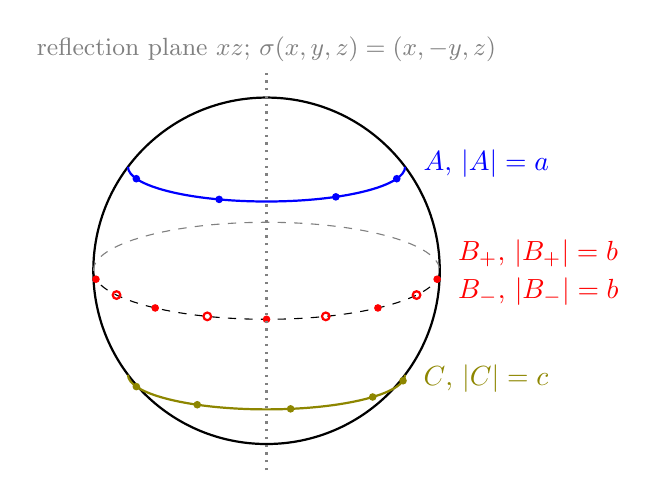
\begin{tikzpicture}[scale=2.2]
  \draw[thick] (0,0) circle (1);
  \draw[dashed] (-1,0) arc (180:360:1 and 0.28);
  \draw[dashed,gray] (-1,0) arc (180:0:1 and 0.28);
  % A layer at z = h
  \draw[blue,thick] (-0.8,0.6) arc (180:360:0.8 and 0.2);
  \foreach \t in {200,250,300,340} \fill[blue] ({0.8*cos(\t)},{0.6+0.2*sin(\t)}) circle (0.022);
  \node[blue,right] at (0.85,0.62) {$A$, $|A|=a$};
  % B layers on the equator: alternating filled/open marks
  \foreach \t in {190,230,270,310,350} \fill[red] ({cos(\t)},{0.28*sin(\t)}) circle (0.022);
  \foreach \t in {210,250,290,330} \draw[red,thick] ({cos(\t)},{0.28*sin(\t)}) circle (0.022);
  \node[red,right] at (1.05,0.1) {$B_+$, $|B_+|=b$};
  \node[red,right] at (1.05,-0.12) {$B_-$, $|B_-|=b$};
  % C layer at z = -h
  \draw[olive,thick] (-0.8,-0.6) arc (180:360:0.8 and 0.2);
  \foreach \t in {200,240,280,320,350} \fill[olive] ({0.8*cos(\t)},{-0.6+0.2*sin(\t)}) circle (0.022);
  \node[olive,right] at (0.85,-0.62) {$C$, $|C|=c$};
  % reflection plane
  \draw[gray,dotted,thick] (0,-1.15) -- (0,1.15);
  \node[gray,above] at (0,1.15) {\small reflection plane $xz$;\ $\sigma(x,y,z)=(x,-y,z)$};
\end{tikzpicture}
\caption{Schematic $\Ctwo$-layer realizer of type $(a,b,c)$. The reflection
$\sigma$ fixes the $A$- and $C$-layers setwise and exchanges the two
alternating equatorial sheets $B_+$ (filled) and $B_-$ (open).}
\label{fig:schematic}
\end{figure}

\begin{lemma}[Layer disjointness]\label{lem:disjoint}
The four layers $A$, $B_+$, $B_-$, and $C$ are pairwise disjoint.
\end{lemma}

\begin{proof}
The layers $A$, $B_+\cup B_-$, and $C$ have distinct $z$-coordinates $h$,
$0$, and $-h$, so only $B_+$ and $B_-$ require attention. If a point of
$B_+$ equaled a point of $B_-$, then for some integers
$0\le i,j\le b-1$,
\[
\frac{i}{b}+\frac{1}{4b} \;\equiv\; \frac{j}{b}-\frac{1}{4b} \pmod 1,
\]
equivalently $i-j+\tfrac12 \in b\,\mathbb Z$, which is impossible because
the left side is a non-integer half-integer while
$b\,\mathbb Z\subseteq\mathbb Z$.
\end{proof}

\begin{lemma}[Equivariance]\label{lem:equiv}
The reflection $\sigma(x,y,z)=(x,-y,z)$ satisfies
\[
\sigma(A)=A,\quad \sigma(C)=C,\quad \sigma(B_+)=B_-,\quad \sigma(B_-)=B_+ .
\]
\end{lemma}

\begin{proof}
This is phase reversal (Lemma~\ref{lem:phase}) applied to the phases $0$,
$\tfrac{1}{4b}$, and $-\tfrac{1}{4b}$.
\end{proof}

\begin{lemma}[Alternating equatorial layer]\label{lem:alt}
The union $B_+\cup B_-$ is the regular equatorial $2b$-gon
$R\bigl(2b,0,\tfrac{1}{4b}\bigr)$ with its vertices divided into two
alternating classes.
\end{lemma}

\begin{proof}
The phases in $B_+$ are $\tfrac{i}{b}+\tfrac{1}{4b}=\tfrac{4i+1}{4b}$,
$i=0,\dots,b-1$: the odd classes congruent to $1$ modulo $4$. The phases
in $B_-$ are $\tfrac{i}{b}-\tfrac{1}{4b}=\tfrac{4i-1}{4b}$; for
$i=1,\dots,b-1$ this equals $\tfrac{4(i-1)+3}{4b}$, and for $i=0$ it is
congruent modulo $1$ to $\tfrac{4b-1}{4b}=\tfrac{4(b-1)+3}{4b}$. Hence
$B_-$ gives the odd classes congruent to $3$ modulo $4$. Together the two
sets give all phases $\tfrac{2\ell+1}{4b}$, $\ell=0,\dots,2b-1$, which are
exactly the phases of $R\bigl(2b,0,\tfrac1{4b}\bigr)$; the two sheets are
the two alternating classes.
\end{proof}

\begin{lemma}[Exposed vertices on the sphere]\label{lem:exposed}
Let $X\subset S^{d-1}$ be finite with distinct points. Then every point of
$X$ is an exposed vertex of $\Conv(X)$.
\end{lemma}

\begin{proof}
Fix $p\in X$ and consider the linear functional $\ell_p(x)=p\cdot x$. Then
$\ell_p(p)=1$. For any $q\in X$ with $q\ne p$, the Cauchy--Schwarz
inequality gives $p\cdot q<1$, because $p$ and $q$ are distinct unit
vectors. Thus $\ell_p$ has a unique maximum at $p$ on $X$. If $x$ is a
convex combination of points of $X$, then $\ell_p(x)$ is the same convex
combination of the values $\ell_p(q)$; since all values except
$\ell_p(p)$ are strictly less than $1$, equality occurs only at $x=p$.
Hence $p$ is exposed in $\Conv(X)$.
\end{proof}

This is the standard strict-convexity fact (see e.g.\ \cite{ziegler} for
general polytope background); it is stated with proof only to keep the
note self-contained.

\begin{proposition}[General $\Ctwo$ vertex count]\label{prop:count}
The set $G$ above satisfies
\[
|\Vertset(\Conv(G))| \;=\; a+2b+c .
\]
\end{proposition}

\begin{proof}
By layer disjointness (Lemma~\ref{lem:disjoint}) and cardinality
(Lemma~\ref{lem:card}), $G$ has $a+b+b+c$ distinct points, all on $S^2$.
By the exposed-vertex lemma every point is an exposed vertex of
$\Conv(G)$.
\end{proof}

\begin{remark}\label{rem:existence}
The proposition is an existence lemma, not a canonical construction for
arbitrary triples. Its role is to isolate the equivariant mechanism by
which the coefficient pattern $(1,2,1)$ is represented: the middle layer
is realized as two alternating sheets exchanged by $\Ctwo$. The
Pythagorean corridor enters only after this mechanism is fixed.
\end{remark}

\section{Pythagorean counts and their arithmetic context}\label{sec:arith}

For integers $m>n\ge1$, the Euclidean parametrization
\[
a=m^2-n^2,\qquad b=2mn,\qquad c=m^2+n^2
\]
produces Pythagorean triples, and every primitive triple arises (up to
order of the legs) from coprime $m,n$ of opposite parity
\cite{sierpinski}. The corridor of the introduction is the slice
$(m,n)=(k+1,k)$. Recall the classical perimeter formula
\[
a+b+c \;=\; 2m(m+n).
\]

\begin{lemma}[Closed corridor count]\label{lem:corridor}
For every $k\ge1$,
\[
a_k+2b_k+c_k \;=\; 2(k+1)(3k+1).
\]
\end{lemma}

\begin{proof}
$a_k+2b_k+c_k=(2k+1)+4k(k+1)+\bigl(2k(k+1)+1\bigr)=6k^2+8k+2=2(k+1)(3k+1)$.
\end{proof}

\begin{lemma}[General count identities]\label{lem:identities}
For all $m>n\ge1$, with $(a,b,c)$ as above,
\[
a+2b+c \;=\; 2m(m+2n),
\qquad\qquad
a+2b+2c \;=\; (m+n)(3m+n).
\]
\end{lemma}

\begin{proof}
$a+2b+c=(m^2-n^2)+4mn+(m^2+n^2)=2m^2+4mn=2m(m+2n)$, and
$a+2b+2c=(m^2-n^2)+4mn+2(m^2+n^2)=3m^2+4mn+n^2=(m+n)(3m+n)$. Equivalently:
the first is the perimeter plus $b$, the second the perimeter plus $b+c$.
\end{proof}

\begin{remark}[OEIS context; nothing here is new]\label{rem:oeis}
The corridor slice of the first identity gives
$2(k+1)(3k+1)$, which is twice the octagonal number $(k+1)(3k+1)$: the
sequence $16, 42, 80, 130, \dots$ is OEIS \textbf{A139267} (``twice
octagonal numbers $2N(3N-2)$''), our value at $k$ sitting at index
$N=k+1$. The identity itself, in the equivalent form
$\mathrm{oct}(N)=B+(A+C)/2$ for Euclid parameters $(N,N-1)$, is a 2013
comment of J.~M.~Bergot on \textbf{A000567}. The corridor slice of the
second identity gives $(2k+1)(4k+3)$: the sequence $21,55,105,\dots$ sits
in OEIS \textbf{A033567} ($a(N)=(2N-1)(4N-1)$), again at index $N=k+1$;
note that $A033567(0)=1$ and $A033567(1)=3$ are \emph{not} corridor
values. The corridor family itself --- odd first legs, hypotenuse
exceeding the even leg by one --- is explicitly documented in the entries
\textbf{A005408}, \textbf{A046092}, \textbf{A001844} \cite{oeis}.
\end{remark}

\section{Realizer theorems on $S^2$}\label{sec:theorems}

\begin{theorem}[Corridor realizer theorem]\label{thm:corridor}
Let $k\ge1$ and $h\in(0,1)$. Define
\[
A_k=R(a_k,h,0),\quad
B_{k+}=R\Bigl(b_k,0,\tfrac{1}{4b_k}\Bigr),\quad
B_{k-}=R\Bigl(b_k,0,-\tfrac{1}{4b_k}\Bigr),\quad
C_k=R(c_k,-h,0),
\]
and $G_k=A_k\cup B_{k+}\cup B_{k-}\cup C_k$. Then $\sigma(A_k)=A_k$,
$\sigma(C_k)=C_k$, $\sigma(B_{k\pm})=B_{k\mp}$; every point of $G_k$ is an
exposed vertex of $P_k=\Conv(G_k)$; and
\[
|\Vertset(P_k)| \;=\; |G_k| \;=\; a_k+2b_k+c_k \;=\; 2(k+1)(3k+1).
\]
Moreover $P_k$ is full-dimensional in $\mathbb R^3$.
\end{theorem}

\begin{proof}
Equivariance and the vertex count follow from
Proposition~\ref{prop:count} and Lemma~\ref{lem:corridor}. For
full-dimensionality: $a_k\ge3$, so $A_k$ contains three non-collinear
points in the plane $z=h$; since $C_k$ is nonempty and lies in the
distinct plane $z=-h$, the affine span of $G_k$ has dimension three.
\end{proof}

\begin{corollary}[Full Euclidean parametrization]\label{cor:euclid}
Let $m>n\ge1$, $(a,b,c)=(m^2-n^2,2mn,m^2+n^2)$, and $h\in(0,1)$. The same
construction with layer sizes $(a,b,b,c)$ yields a $\Ctwo$-equivariant
vertex realizer with
\[
|\Vertset(P)| \;=\; a+2b+c \;=\; 2m(m+2n),
\]
full-dimensional in $\mathbb R^3$.
\end{corollary}

\begin{proof}
Proposition~\ref{prop:count} applies to arbitrary positive integers
$(a,b,c)$, and $a=m^2-n^2\ge (n+1)^2-n^2=2n+1\ge3$ gives
full-dimensionality as in Theorem~\ref{thm:corridor}. The count is
Lemma~\ref{lem:identities}.
\end{proof}

\section{An integer-layer realizer on $S^3$}\label{sec:s3}

We now iterate the mechanism once, one dimension up, for the coefficient
pattern $(1,2,2,1)$. A vertex count is a cardinality; consequently
\emph{every} layer of any such pattern must have an integer size. The
correct four-dimensional statement therefore carries a freely declared
integer top layer $e\ge1$; no irrational multiple of a layer size (such as
the $c\sqrt2$ of the withdrawn precursor) can occur in a vertex count.

\begin{definition}\label{def:layer4}
For an integer $n\ge1$, parameters $\zeta,w$ with $\zeta^2+w^2<1$, and a
phase $\varphi\in\mathbb R$, define the \emph{latitude circle layer}
\[
R_4(n,\zeta,w,\varphi)=\left\{\Bigl(\rho\cos 2\pi\bigl(\tfrac{i}{n}+\varphi\bigr),\;
\rho\sin 2\pi\bigl(\tfrac{i}{n}+\varphi\bigr),\; \zeta,\; w\Bigr) : i=0,\dots,n-1\right\},
\]
where $\rho=\sqrt{1-\zeta^2-w^2}>0$. Each point lies on $S^3$, and
$|R_4(n,\zeta,w,\varphi)|=n$ by the argument of Lemma~\ref{lem:card}.
We call $(\zeta,w)$ the \emph{signature} of the layer.
\end{definition}

Let $\sigma_4(x,y,z,w)=(x,y,z,-w)$. Since $\sigma_4$ acts only on the last
coordinate,
\[
\sigma_4\bigl(R_4(n,\zeta,w,\varphi)\bigr)=R_4(n,\zeta,-w,\varphi).
\]

Fix positive integers $a,b,c,e$ and parameters
\[
\zeta_a\ne\zeta_e, \qquad t_b,t_c>0, \qquad (\zeta_b,t_b)\ne(\zeta_c,t_c),
\]
all subject to $\zeta^2+w^2<1$ for each layer below. Define
\[
A=R_4(a,\zeta_a,0,0),\qquad E=R_4(e,\zeta_e,0,0),
\]
\[
B_\pm=R_4(b,\zeta_b,\pm t_b,0),\qquad
C_\pm=R_4(c,\zeta_c,\pm t_c,0),
\]
and $G=A\cup B_+\cup B_-\cup C_+\cup C_-\cup E$.

\begin{lemma}[Disjointness by signatures]\label{lem:sig}
The six layers are pairwise disjoint.
\end{lemma}

\begin{proof}
Under the stated parameter conditions the six signatures
$(\zeta_a,0)$, $(\zeta_e,0)$, $(\zeta_b,\pm t_b)$, $(\zeta_c,\pm t_c)$ are
pairwise distinct: the two fixed layers differ in $\zeta$; each mirror
pair differs in the sign of $w\ne0$; the same-sign $B/C$ pairs differ
because $(\zeta_b,t_b)\ne(\zeta_c,t_c)$; the mixed-sign $B/C$ pairs differ
in the sign of $w$, since $t_b>0>-t_c$ and $-t_b<0<t_c$; and fixed layers
differ from mirror layers because $t_b,t_c>0$. Points in layers with
distinct signatures differ in their last two coordinates.
\end{proof}

\begin{remark}
On $S^2$ the two $B$-sheets shared the same latitude and the disjointness
argument needed the half-integer phase computation of
Lemma~\ref{lem:disjoint}; on $S^3$ each layer carries its own signature,
so no phase argument is needed. The price is that the mirror pairs are
parallel $n$-gons rather than interleaved sheets of a single $2n$-gon.
\end{remark}

\begin{theorem}[Integer-layer realizer on $S^3$]\label{thm:s3}
With the data above, $\sigma_4$ fixes $A$ and $E$ setwise (indeed
pointwise) and exchanges $B_+\leftrightarrow B_-$ and
$C_+\leftrightarrow C_-$; every point of $G$ is an exposed vertex of
$P=\Conv(G)$; and
\[
|\Vertset(P)| \;=\; a+2b+2c+e .
\]
Moreover $P$ is full-dimensional in $\mathbb R^4$ whenever $a\ge3$.
In particular, for a Pythagorean triple from Euclid parameters $m>n\ge1$
and any declared integer $e\ge1$,
\[
|\Vertset(P)| \;=\; (m+n)(3m+n)+e .
\]
\end{theorem}

\begin{proof}
Equivariance is the displayed action of $\sigma_4$ on signatures.
Disjointness is Lemma~\ref{lem:sig}, so $|G|=a+2b+2c+e$ with all points
distinct on $S^3$; the exposed-vertex lemma (Lemma~\ref{lem:exposed},
stated for $S^{d-1}$) gives the vertex count. For full-dimensionality:
$A$ contains three non-collinear points in the $2$-plane
$\{z=\zeta_a,\,w=0\}$; a point of $E$ (with $z=\zeta_e\ne\zeta_a$, $w=0$)
raises the affine dimension to three inside the hyperplane $w=0$; a point
of $B_+$ (with $w=t_b\ne0$) raises it to four. The Pythagorean count is
Lemma~\ref{lem:identities}, and $a=m^2-n^2\ge3$ always holds.
\end{proof}

\begin{remark}[A symmetric choice of top layer]\label{rem:topchoice}
The choice $e=a$ gives
\[
a+2b+2c+a \;=\; 2(a+b+c) \;=\; 4m(m+n),
\]
twice the perimeter --- the pattern $(1,2,2,1)$ becomes the ``doubled''
pattern $2(1,1,1)$ on the triple itself.
\end{remark}

\begin{figure}[ht]
\centering
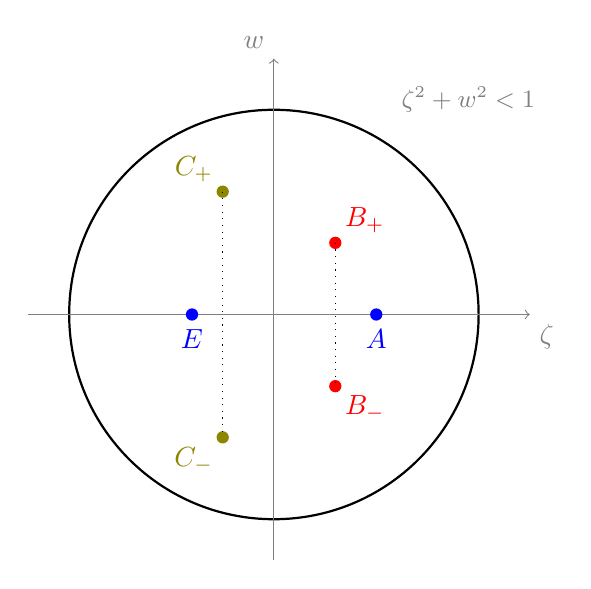
\begin{tikzpicture}[scale=2.6]
  \draw[thick] (0,0) circle (1);
  \draw[gray,->] (-1.2,0) -- (1.25,0) node[below right] {$\zeta$};
  \draw[gray,->] (0,-1.2) -- (0,1.25) node[above left] {$w$};
  \fill[blue] (0.5,0) circle (0.03) node[below=2pt] {$A$};
  \fill[blue] (-0.4,0) circle (0.03) node[below=2pt] {$E$};
  \fill[red] (0.3,0.35) circle (0.03) node[above right=0pt] {$B_+$};
  \fill[red] (0.3,-0.35) circle (0.03) node[below right=0pt] {$B_-$};
  \fill[olive] (-0.25,0.6) circle (0.03) node[above left=0pt] {$C_+$};
  \fill[olive] (-0.25,-0.6) circle (0.03) node[below left=0pt] {$C_-$};
  \draw[dotted] (0.3,0.35) -- (0.3,-0.35);
  \draw[dotted] (-0.25,0.6) -- (-0.25,-0.6);
  \node[gray] at (0.95,1.05) {\small $\zeta^2+w^2<1$};
\end{tikzpicture}
\caption{Signature diagram of the $S^3$ construction: each latitude circle
layer is a point in the open unit disk of the $(\zeta,w)$-plane. The
reflection $\sigma_4$ acts as $w\mapsto-w$: the fixed layers $A,E$ sit on
the axis, the doubled layers form mirror pairs.}
\label{fig:signature}
\end{figure}

\section{A small boundary atlas}\label{sec:atlas}

The theorems above concern vertex counts only; edge and face numbers are
\emph{not} determined by them and belong to the specific realizer. This
section records, purely descriptively, the computed boundary data of the
corridor realizers $P_k=\Conv(G_k)$ of Theorem~\ref{thm:corridor}. The
computation takes the exact construction (phases $0$, $\pm\tfrac1{4b_k}$,
$0$), merges the triangulated hull facets into true planar faces, counts
$E=\tfrac12\sum_{\text{faces}}(\text{face size})$, and verifies Euler's
relation $V-E+F=2$ as a consistency check. For every
$k=1,\dots,20$ and every tested height $h\in\{0.2,\,0.5,\,0.8\}$ the
resulting $(V,E,F)$ and face-size profile were identical across the three
heights; all $60$ runs pass the vertex-count and Euler checks.

\begin{center}
\begin{tabular}{rrrrrl}
\toprule
$k$ & $(a_k,b_k,c_k)$ & $V$ & $E$ & $F$ & face profile \\
\midrule
 1 & $(3,4,5)$        & $16$  & $38$   & $24$   & $21$ triangles, $2$ quads, $c$-gon cap \\
 2 & $(5,12,13)$      & $42$  & $106$  & $66$   & $62$ triangles, $2$ quads, $a$-, $c$-gon caps \\
 3 & $(7,24,25)$      & $80$  & $206$  & $128$  & $124$ triangles, $2$ quads, caps \\
 4 & $(9,40,41)$      & $130$ & $338$  & $210$  & $206$ triangles, $2$ quads, caps \\
 5 & $(11,60,61)$     & $192$ & $502$  & $312$  & $308$ triangles, $2$ quads, caps \\
 6 & $(13,84,85)$     & $266$ & $698$  & $434$  & $430$ triangles, $2$ quads, caps \\
 7 & $(15,112,113)$   & $352$ & $926$  & $576$  & $572$ triangles, $2$ quads, caps \\
 8 & $(17,144,145)$   & $450$ & $1186$ & $738$  & $734$ triangles, $2$ quads, caps \\
 9 & $(19,180,181)$   & $560$ & $1478$ & $920$  & $916$ triangles, $2$ quads, caps \\
10 & $(21,220,221)$   & $682$ & $1802$ & $1122$ & $1118$ triangles, $2$ quads, caps \\
\bottomrule
\end{tabular}
\end{center}

The structure visible in the profile column is uniform over the computed
range: the plane $z=h$ supports the regular $a_k$-gon of $A_k$ as a top
cap and $z=-h$ supports the $c_k$-gon of $C_k$ as a bottom cap (for
$k=1$ the top cap is a triangle and is counted among the triangles);
exactly two quadrilateral faces occur, sitting astride the reflection
plane --- note that any two $\sigma$-paired points span translation
vectors parallel to the $y$-axis, so two mirror pairs are always
coplanar, and at the two seams of the configuration such a quadruple is
extremal in the computed range; all remaining faces are triangles.

\begin{remark}[No claim]\label{rem:noclaim}
Everything in this section is computed data for the specific realizers at
the tested parameters ($k\le 20$, three heights). For the record, for all
computed $k$ ($1\le k\le 20$, all three heights) the data fit
$E=16k^2+20k+2$ and $F=10k^2+12k+2$ (consistent with Euler and
$V=6k^2+8k+2$). We make
\emph{no} claim that the face structure, the fits, or the
$h$-independence persist beyond the computed range, and we do not pursue
proofs; $f$-vectors of the general construction are outside the scope
fixed in Section~\ref{sec:intro}.
\end{remark}

\section{Context, prior art, and terminology}\label{sec:context}

\paragraph{Prior art.} The arithmetic layer of this note is known or
elementary: A139267 (count sequence), the Bergot comment on A000567
(corridor identity), A001844/A046092/A005408 (the family), and the
perimeter formula from which Lemma~\ref{lem:identities} is one line. The
geometric layer rests on the textbook exposedness fact
(Lemma~\ref{lem:exposed}); realizing \emph{any} prescribed number of hull
vertices by points on a sphere is therefore trivial as pure existence. The
residual content of the constructions is only the explicit equivariant
layer bookkeeping. Convex hulls of orbits of finite groups are studied in
much greater generality in the orbit-polytope literature
\cite{frieseladisch,matteo}; nothing in this note adds to that theory.

\paragraph{Terminology.} ``Realization'' has an established, different
meaning in rigidity theory (embeddings of graphs on spheres, e.g.\
counting realizations of Laman graphs \cite{laman}). Here \emph{realizer}
means only: a configuration whose convex hull attains a prescribed vertex
count with prescribed equivariant layer structure.

\section{Remarks and limitations}\label{sec:limits}

Different choices of the parameters ($h$; the signatures; the phases) yield
non-congruent realizers with the same vertex count, so the results are
equivariant realizability statements, not uniqueness statements. The
constructions give vertex realizers, not $f$-vector theorems: edge and face
counts are not determined here. The general propositions are existence
lemmas; they are not canonical or natural in any categorical sense. And, as
stated throughout, none of the mathematical content is new; the note is a
consolidation with corrected statements and fixed arithmetic context.

\appendix

\section{Computational reproducibility}\label{app:comp}

The proofs above are independent of computation; the following
implementation checks accompany the project.

\begin{center}
\begin{tabular}{lllll}
\toprule
Script & Cases & Counts & Checks & Result \\
\midrule
\texttt{verify\_c2\_realizer.py} & $k=1,\dots,20$ & $16$ -- $2562$ &
hull count $=2(k{+}1)(3k{+}1)$ & $20/20$ \\
\texttt{verify\_s3\_realizer.py} & $50$ runs ($48$ distinct) & $22$ -- $1300$ &
hull count, disjointness, $\sigma_4$ & $50/50$ \\
\texttt{check\_oeis\_prior\_art.py} & $11$ checks & --- &
identities, OEIS terms, offsets & $11/11$ \\
\texttt{atlas\_boundary.py} & $k\le20$, $3$ heights & --- &
merged $f$-vectors, Euler & $60/60$ \\
\bottomrule
\end{tabular}
\end{center}

The $S^2$ script rebuilds $G_k$ and checks
$|\Vertset(\Conv(G_k))|=2(k+1)(3k+1)$ for $k=1,\dots,20$
(\texttt{results/baseline\_k1\_20.csv}). The $S^3$ script checks
Theorem~\ref{thm:s3} on the corridor $k=1,\dots,12$ with
$e\in\{1,\,a_k,\,7\}$ and on six further non-corridor Euclid pairs with
$e\in\{1,5\}$ ($50$ runs, $48$ distinct cases; two duplicates arise at
$(m,n)=(4,3)$, where $a_k=7$ and the pair also appears in the general
list), verifying layer disjointness, $\sigma_4$-equivariance, and
the four-dimensional hull vertex count
(\texttt{results/s3\_realizer\_check.csv}). The OEIS script re-derives the
identities of Lemma~\ref{lem:identities} symbolically and diffs the
archived OEIS entries against the computed baselines
(\texttt{results/oeis\_prior\_art\_check.txt}). The atlas script produces
the merged-face data of Section~\ref{sec:atlas}
(\texttt{results/atlas\_boundary.csv}). These computations are
implementation checks and descriptive data, not ingredients in the
proofs.

\begin{thebibliography}{9}

\bibitem{oeis}
OEIS Foundation Inc.\ (2026), \emph{The On-Line Encyclopedia of Integer
Sequences}, \texttt{https://oeis.org}. Entries A000567, A001844, A005408,
A033567, A046092, A139267.

\bibitem{sierpinski}
W.~Sierpi\'nski, \emph{Pythagorean Triangles}, Graduate School of Science,
Yeshiva University, New York, 1962 (Dover reprint, 2003).

\bibitem{ziegler}
G.~M.~Ziegler, \emph{Lectures on Polytopes}, Graduate Texts in
Mathematics 152, Springer, New York, 1995.

\bibitem{frieseladisch}
E.~Friese and F.~Ladisch, Affine symmetries of orbit polytopes,
\emph{Adv.\ Math.} \textbf{288} (2016), 386--425.

\bibitem{matteo}
N.~Matteo, Two-orbit convex polytopes and tilings,
arXiv:1403.2125.

\bibitem{laman}
M.~Gallet, G.~Grasegger, and J.~Schicho, Counting realizations of Laman
graphs on the sphere, arXiv:1903.01145.

\end{thebibliography}

\end{document}
